\documentclass[14pt,fleqn]{extarticle}
\RequirePackage{prepwell-eng}

\previewoff

\begin{document} 
\begin{snippet}
    \correct
    
    \[\prob{A\cup B} = \prob{A\cap B} + \prob{A\cap B'} + \prob{A'\cap B} \]
    
    \reason
    
    Given two events $A$ and $B$, the following figures show 
    what $A\cap B, A\cap B'$ and $A'\cap B$ look like 
    
    \begin{center}
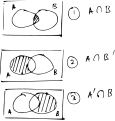
\includegraphics[scale=1.4]{98-A.svg}
\end{center}

And one can see that if the three areas \underline{are added together} then one will 
get $A\cup B$. Which is why 
\[\prob{A\cup B} = \prob{A\cap B} + \prob{A\cap B'} + \prob{A'\cap B} \]
\end{snippet} 
\end{document} 
